\documentclass[lualatex,12pt,ja=standard]{bxjsreport}

\author{小森理央}
\title{可換砂山モデル}
\date{2023年1月13日}

\usepackage{amssymb}
\usepackage{amsmath}
\usepackage{tikz}
\usepackage{pgf}
\usepackage[]{hyperref}
\usepackage{graphicx}
\usepackage{float}

\begin{document}
\maketitle

\tableofcontents

%\chapter{導入}
\chapter{序}
可換砂山モデル(Abelian sandpile model)はBak,Tang,Wiesenfeld\cite{BTW}に
より導入された統計物理学のモデルであり、
{\em 自己組織化臨界現象}と呼ばれる性質をもつ例としてよく知られている。
砂山モデルは任意の無向グラフ上で定義されるが、
特に詳しく研究されてきたのは2次元の正方格子グラフ上の
ものである。
例えば、正方格子上の砂山モデルをコンピュータでシミュレートすると、
{\em 雪崩}の規模と頻度を記録するとそれが
冪乗則に従うことが知られており、一点に砂粒を投下し続けると
12角形上に砂粒が広がることが知られている。
本研究の主な目的はペンローズタイル張りにおいて砂山モデルを
コンピュータでシミュレートすることにより、その
性質を調べることである。

%正方格子では雪崩の規模と頻度がべき乗則に従うことがわかっている。ペンローズタイルではどのような動きになるのか確かめる。

\chapter{可換砂山モデル}
%可換砂山モデルは1987年にBak,Tang,Wiesenfeldによって導入され、砂山の雪崩の規模と頻度の関係はべき乗則に従うことが明らかになっている。また系が任意%の初期状態から臨界状態へ到達し、臨界状態であるときに衝撃をわずかでも与えると系が影響を受ける、自己組織化臨界現象を示すモデルとして知られている。

可換砂山モデルは1987年にBak,Tang,Wiesenfeldによって導入された統計物理学の
モデルであり、
{\em 自己組織臨界現象}が観測出来るモデルとして有名である。
このモデルの定義を下記に与える。

可換砂山モデルは任意のグラフに対して定義出来る。
$G=(V\cup\{s\},E)$を無向グラフとする。
$s$は沈点と呼ばれる任意の頂点と道でつながる頂点である。
{\em 砂山配置}$\sigma$とは写像$\sigma: V\to {\mathbb Z}$である。
つまり、$\sigma$は各頂点に砂粒の負の個数も含めた個数を割り当てたものである。
配置全体の集合を${\rm Conf}(G)$と
表す。つまり${\rm Conf}(G)={\mathbb Z}^V$である。
$v\in V$に対して$\sigma(v)\geq \deg_G(v)$であるとき,
$v$は$\sigma$において{\em 不安定}であるという。
不安定でない頂点は{\em 安定}であるという。
すべての頂点$v$が安定であるとき$\sigma$は{\em 安定な配置}であるという。
配置$\sigma$に対して,新しい配置$\sigma'$を
\[
 \sigma'(w) = \begin{cases}
	      \sigma(v)-\deg_G(v) & w = v\\
	      \sigma(w)+1 & w\sim v\\
	      \sigma(w)& {その他}
	     \end{cases}
\]
と定める。写像$\sigma\mapsto \sigma'$を$v$における{\em 発火}(fireまたはtopple)と呼び、
$\sigma\stackrel{v}{\to}\sigma'$と表す。
発火する頂点が不安定であるとき、その発火は$legal$であるという。
頂点の列$v_1, v_2, \ldots, v_l$に対して、
\[
 \sigma \stackrel{v_1}{\to} \sigma_1 \stackrel{v_2}{\to}   \cdots
  \stackrel{v_l}{\to} \sigma_l
\]
であるとする。
このとき、任意の$l$次の置換$i_1i_2\cdots i_l$に対して、
\[
 \sigma \stackrel{v_{i_1}}{\to} \sigma'_1 \stackrel{v_{i_2}}{\to}   \cdots
  \stackrel{v_{i_l}}{\to} \sigma'_l
\]
ならば、$\sigma_l = \sigma'_l$が成立する。
つまり、発火する頂点の順序によらず,各頂点での発火回数が
等しければ,最終的に得られる配置は一定で変わらない。
これが可換と呼ばれる理由である。
沈点への砂粒の流出があるため、どのような配置$\sigma$もlegalな発火を有限回繰り返すことにより,
安定な配置に変化する。
この安定配置は$\sigma$に対して一意に定まり、
これを$\sigma^\circ$と表し$\sigma$の{\em 安定化}と呼ぶ。
非負の安定配置全体を${\rm Stab}(G)$と表す。
$v\in V$に対して
\[
E_v:{\rm Conf}(G)\ni \sigma\mapsto \left(\sigma + 1_v\right)^\circ\in {\rm Stab}(G)
\]
を{\em 追加作用素}と呼ぶ。ただし、$1_v(w) = \delta_{v,w}$(クロネッカー記号)である。
つまり,$E_v$は$v$上に一つ砂粒を加え、安定化する作用素である。
$X_1, X_2, \ldots$は$V$上に一様に分布する独立な確率変数列であるとする。
$\xi_0\in {\rm Stab}(G)$に対して、
\[
 \xi_k = E_{X_k}E_{X_{k-1}}\cdots E_{X_1} \xi_0
\]
と定めると、$\xi_0,\xi_1,\xi_2,\ldots$は${\rm Stab}(G)$上のマルコフ連鎖となる。
これが可換砂山モデルである。つまり、可換砂山モデルはランダムに選ばれた頂点上に
砂粒を一つ落として、安定化する操作を繰り返すときの砂山の変化の様子を
モデル化したものである。このマルコフ連鎖の再帰状態全体${\mathcal S}_G$は
以下に定める加法$\stackrel{*}{+}$に関してアーベル群を成す。
\[
 \sigma \stackrel{*}{+} \tau \stackrel{def}{=}
 \left(\sigma + \tau\right)^\circ
\]
${\mathcal S}_G$を{\em 砂山群}と呼ぶ。よって、このマルコフ連鎖を
群${\mathcal S}_G$上のランダムウォークと
みなせ、その定常分布$\nu_G$が${\mathcal S}_G$上の一様分布であることが分かる。
この定常分布$\nu_G$のもとでの配置そのものや、$E_X$が引き起こす発火の列、
雪崩(avalanche)の範囲や形、個数がどのように分布するのかが
知りたい。
こうした分布がいろいろな例において冪乗則で近似出来ることが知られており、
その指数({\em 臨界指数})を評価・決定することが数理物理的視点からの
\underline{中心的な問い}の一つである。


\chapter{正方格子グラフにおける計算機実験}

\section{正方格子グラフ}
本校で正方格子グラフ$G_{m,n}$とは
次のように定義される無向グラフ$G=(V\cup\{s\},E)$である。
頂点集合$V$は
\[
 V = \left\{(x,y)\,|\, x\in {0,1,\ldots,m-1}, y\in \{0,1,\ldots,n-1\}\right\}
\]
と定義される。
また辺集合$E$は
\begin{eqnarray*}
 E & = & \{\{v,w\}\,|\, v,w\in V, v-w \in\{(\pm 1,0), (0,\pm 1)\}\} \cup \\
 & & ~~~~ \{\{s,v\}\,|\, v=(x,y), x\in \{0,m-1\}または y\in\{0,n-1\}\}
\end{eqnarray*}
と定義される。つまり、$G$は
座標平面上で$x$座標$y$座標がともに整数である
点の長方形状にならんだ部分集合を頂点集合として、
それらの最近接の頂点同士を結ぶ辺に加え、周辺の頂点を
すべて一本の辺で沈点$s$と結ぶ。

\section{実験}
図\ref{fig:experiment1}は$m=n=200$とした正方格子グラフ$G_{200,200}$
における実験の結果である。
縦方向と横方向にマスが200個ずつ並べられている正方格子を考え、計4万個のマスのどこかに無作為に砂粒を1粒ずつ落とし、この動作を1万回から実施回数を増やしていき、100万回まで行う。ある一つのマスに4個目の砂粒が落とされたとき、そのマスの砂粒の山は崩れ、隣接する四方向に一粒ずつ移動する。また一番外側にあるマスに砂粒が落ちたときは存在する隣接のマスへのみ一粒ずつ移動させ、残りの砂粒の分はそのマスにもとどまらず消滅させることにし、任意のマスに4粒目の砂粒が落ちたときは該当のマスの砂粒をゼロにする。以上の動作を繰り返し行い、各回数繰り返した後の砂粒の積み重ねをヒートマップで可視化した。
上の図は1万回繰り返した時のヒートマップである。ヒートマップでは砂粒が0個のマスは黒色で表示され、砂粒が多くなるにつれて赤色や黄色に変化する。

\begin{figure}[H]
 \begin{center}
  \includegraphics[width=10cm]{heatmap_10000.pdf}
  \includegraphics[width=10cm]{heatmap_100000.pdf}
  \caption{$G_{200,200}$における実験}
  \label{fig:experiment1}
 \end{center}
\end{figure}


(この頻度と規模を段階にわけて表にした図を載せたい)

\subsection{冪乗則}
規模と頻度の対数をそれぞれとってグラフにすると図\ref{fig:experiment2}のようになる。
途中(詳しく?)までは直線上に乗るが、一定を超えると急降下し外れてしまう。
\begin{figure}[H]
 \begin{center}
\includegraphics[width=10cm]{Rplot_square.pdf}
  \caption{雪崩の規模と頻度の関係}
  \label{fig:experiment2}
 \end{center}
\end{figure}

\subsection{パターン形成}
一点に砂粒を投下し続ける実験を行った。
図$\ref{fig:onePoint40000}$から図$\ref{fig:onePoint70000}$
は順に一点に4万粒、5万粒、6万粒、7万粒を投下した
結果である。
実験画像からは特有のパターンが伺えるが、これが
なぜ生じるのか、またこのパターンをどのように数学的に
記述するのかは分からないままである。
また、砂粒は投下点を中心に
12角形状に広がっていくことが伺える。
やはり、なぜこのような形状を取るのかは分かっていない。

\begin{center}
 \begin{figure}[H]
  \begin{center}
   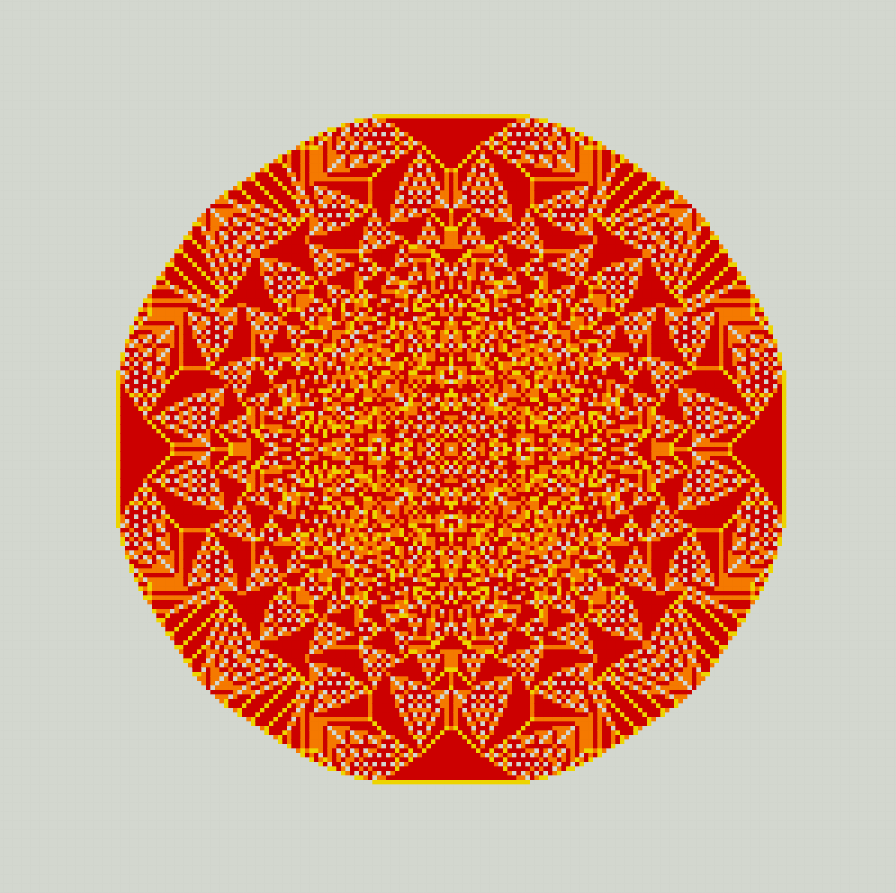
\includegraphics[bb=0 0 896 893,clip,width=8cm]{figures/onepoint40000.png}
  \end{center}
  \caption{1点に砂粒を投下して安定化させた様子:4万粒}
  \label{fig:onePoint40000}
 \end{figure}
\end{center}

\begin{center}
 \begin{figure}[H]
  \begin{center}
   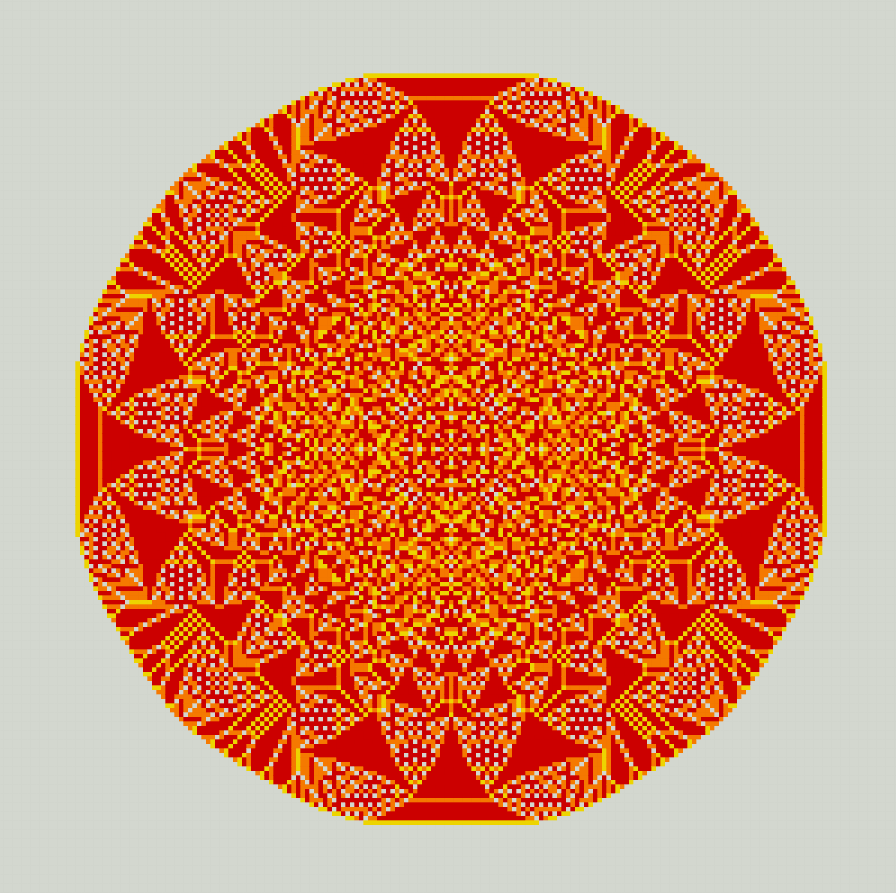
\includegraphics[bb=0 0 896 893,clip,width=8cm]{figures/onePoint50000.png}
  \end{center}
  \caption{1点に砂粒を投下して安定化させた様子:5万粒}
 \end{figure}
\end{center}

\begin{center}
 \begin{figure}[H]
  \begin{center}
   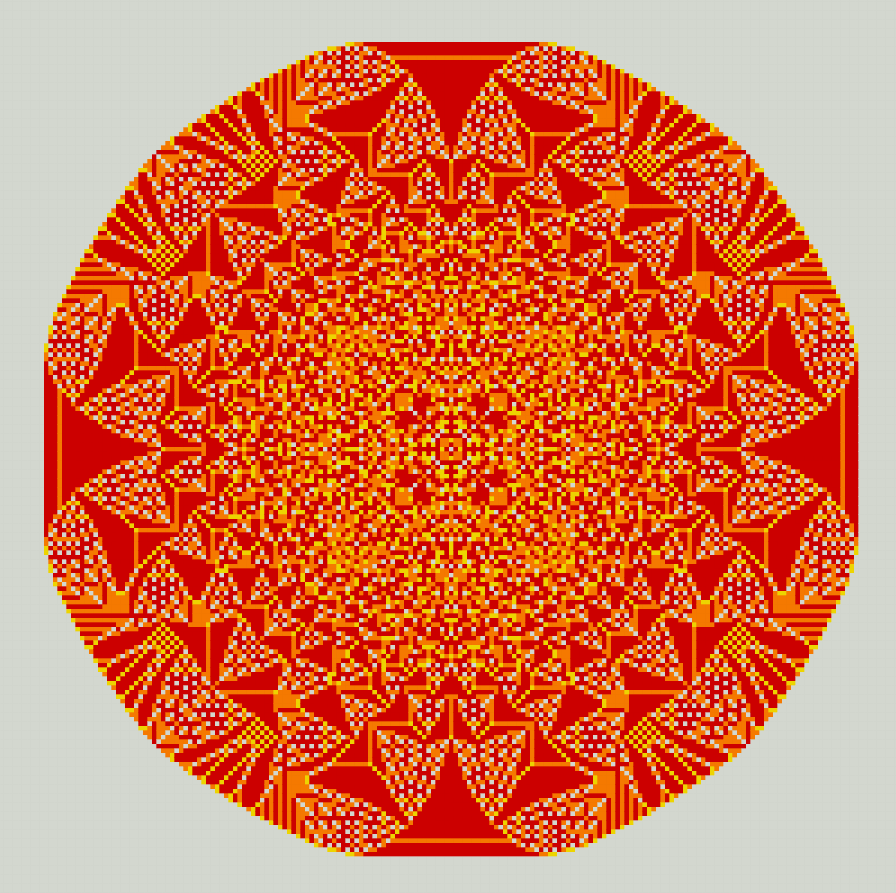
\includegraphics[bb=0 0 896 893,clip,width=8cm]{figures/onePoint6000.png}
  \end{center}
  \caption{1点に砂粒を投下して安定化させた様子:6万粒}
 \end{figure}
\end{center}

\begin{center}
 \begin{figure}[H]
  \begin{center}
   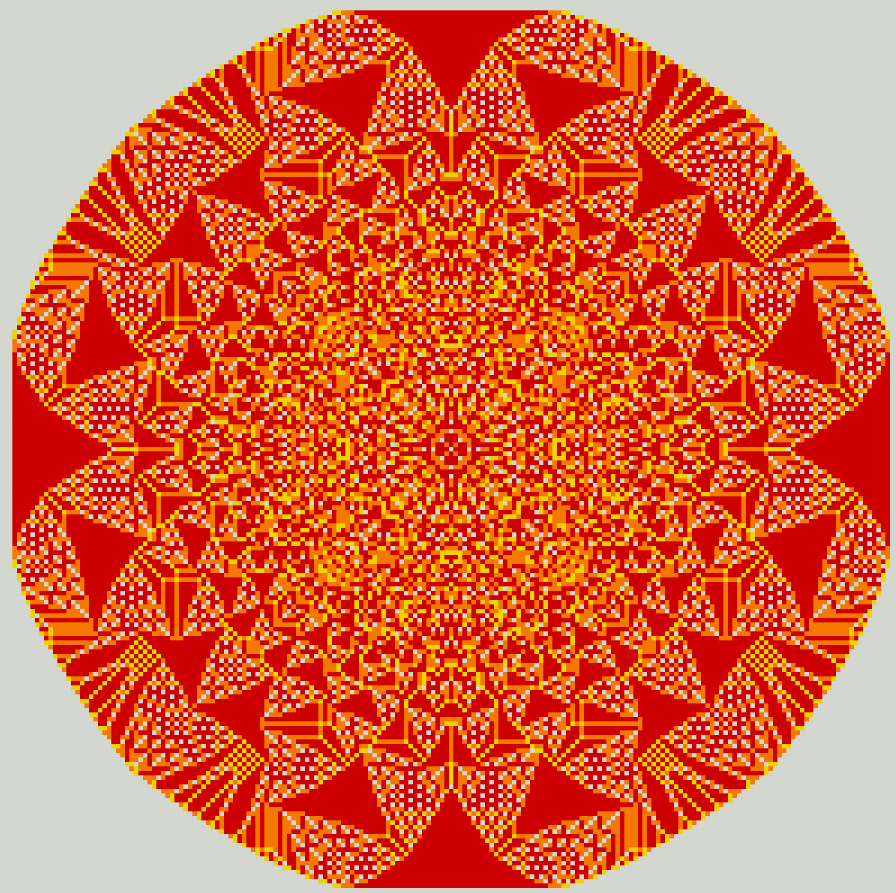
\includegraphics[bb=0 0 896 893,clip,width=8cm]{figures/onePoint70000.png}
  \end{center}
  \caption{1点に砂粒を投下して安定化させた様子:7万粒}
  \label{fig:onePoint70000}
 \end{figure}
\end{center}

%\chapter{ペンローズタイルモデル}
\chapter{ペンローズタイル張り上の砂山モデル}

\section{ペンローズタイル張り}
ペンローズタイル張りはノーベル物理学賞受賞者の
ロジャー・ペンローズ氏が発見した準周期性と呼ばれる
特徴を持つ二次元平面のタイル張りである。
その構成方法を簡単に述べる。

\begin{description}
 \item[初期配置]
	    下記のように10枚の三角形が原点を共有するようにに配置する。
	    各三角形には向きがあることに注意する。
	    \begin{center}
	     \begin{figure}[H]
	      \begin{center}
	       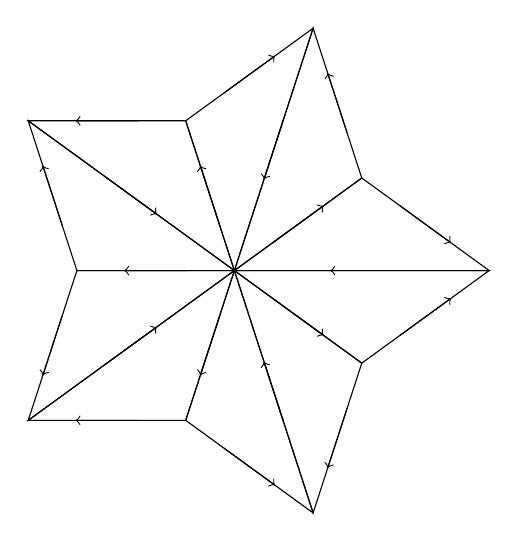
\begin{tikzpicture}[scale=2]
		\draw[->,>=latex] (0,0) -- ({2*cos(36)},0) -- ({cos(36)},{sin(36)})--cycle;
		\draw[->,>=latex] (0,0) -- ({2*cos(36)},0) -- ({cos(36)},{-sin(36)})--cycle;
		\draw[->] ({cos(36)+0.2},0) -- ({cos(36)-0.2},0);
		\draw[->] ({cos(36)*0.3},{sin(36)*0.3}) -- ({cos(36)*0.7},{sin(36)*0.7});
		\draw[->] ({cos(36)},{sin(36)}) ++ ({cos(36)*0.3},{-sin(36)*0.3}) -- ++ ({cos(36)*0.4},{-sin(36)*0.4});
		\draw[->] ({cos(36)},{-sin(36)}) ++ ({cos(36)*0.3},{sin(36)*0.3}) -- ++ ({cos(36)*0.4},{sin(36)*0.4});
		\foreach \i in {1,...,4}{
		\begin{scope}[rotate={\i*72}]
		\draw[->,>=latex] (0,0) -- ({2*cos(36)},0) -- ({cos(36)},{sin(36)})--cycle;
		\draw[->,>=latex] (0,0) -- ({2*cos(36)},0) -- ({cos(36)},{-sin(36)})--cycle;
		\draw[->] ({cos(36)+0.2},0) -- ({cos(36)-0.2},0);
		\draw[->] ({cos(36)*0.3},{sin(36)*0.3}) -- ({cos(36)*0.7},{sin(36)*0.7});
		\draw[->] ({cos(36)},{sin(36)}) ++ ({cos(36)*0.3},{-sin(36)*0.3}) -- ++ ({cos(36)*0.4},{-sin(36)*0.4});
		\draw[->] ({cos(36)},{-sin(36)}) ++ ({cos(36)*0.3},{sin(36)*0.3}) -- ++ ({cos(36)*0.4},{sin(36)*0.4});
		\end{scope}
		}
	       \end{tikzpicture}
	      \end{center}
	     \end{figure}
	    \end{center}


 \item[細分] 
	    ペンローズタイル張りを構成する途中で2つのタイプの三角形
	    $A$と$B$が現れる。
	    タイプ$A$は等辺が長さ$\tau = \frac{1+\sqrt{5}}{2}$で
	    底辺が長さ$1$の二等辺三角形であり、
	    タイプ$B$は等辺の長さが$1$で底辺の長さが$\tau$の二等辺三角形である。
	    それぞれを細分するルールを下の図に示す。

	    \begin{center}
	     \begin{figure}[H]
	      \begin{center}
	       \begin{tikzpicture}[scale=3]
		\draw[->,>=latex] (0,0) -- ({2*cos(36)},0) -- ({cos(36)},{sin(36)})--cycle;
		\draw[->] ({cos(36)+0.2},0) -- ({cos(36)-0.2},0);
		\draw[->] ({cos(36)*0.3},{sin(36)*0.3}) -- ({cos(36)*0.7},{sin(36)*0.7});
		\draw[->] ({cos(36)},{sin(36)}) ++ ({cos(36)*0.3},{-sin(36)*0.3}) -- ++ ({cos(36)*0.4},{-sin(36)*0.4});
		\draw ({cos(36)},0.2) node {$B$};
		\draw[line width = 3, ->, >=latex](2,0.2) -- (2.4,0.2);
		\begin{scope}[xshift=3cm]
		\draw[->,>=latex] (0,0) -- ({2*cos(36)},0) -- ({cos(36)},{sin(36)})--cycle;
		 \draw[] (1,0) -- ({cos(36)}, {sin(36)});
		 \draw[->] (0.3,0) -- (0.7,0);
		 \draw[->] ({0.3*cos(36)},{0.3*sin(36)}) -- ({0.7*cos(36)},{0.7*sin(36)});
		 \draw[->] ({cos(36)},{sin(36)}) ++ ({cos(36)*0.3},{-sin(36)*0.3}) -- ++ ({cos(36)*0.4},{-sin(36)*0.4});
		 \draw[->] (1,0) ++ ({cos(108)*0.2},{sin(108)*0.2}) -- ++({cos(108)*0.2},{sin(108)*0.2});
		\end{scope}
		\begin{scope}[yshift=1cm,xshift=0.3cm]
		 \draw (0,0) --  (1,0) -- ({1/2},{tan(72)/2}) -- cycle;
		 \draw[->] ({cos(72)*0.7},{sin(72)*0.7}) -- ({cos(72)*0.4},{sin(72)*0.4});
		 \draw[->] ({1/2},{tan(72)/2}) ++ ({cos(72)},{-sin(72)}) -- ++({cos(72)*0.2},{-sin(72)*0.2});
		 \draw[->] (0.7,0) -- (0.4,0);
		 \draw[line width = 3, ->, >=latex](1.6,0.2) -- ++(0.4,0);
		 \draw ({1/2)},0.2) node {$A$};
		\begin{scope}[xshift=3cm]
		 \draw (0,0) --  (1,0) -- ({1/2},{tan(72)/2}) -- cycle;
		 \draw[->] (1,0) -- ++({-1/2*0.3},{tan(72)/2*0.3});
		 \draw[->] (1,0) -- (0.5,0);
		 \draw[->] (0,0) -- ++({1/2*0.3},{tan(72)/2*0.3});
		 \draw[->] (0,0) -- ++({1/2*0.8},{tan(72)/2*0.8});
		 \draw (1,0) -- ++({cos(144)},{sin(144)}) -- ({1+cos(108)},{sin(108)});
		 \draw[->] (1,0) -- ++({cos(144)*0.5},{sin(144)*0.5});
		 \draw[->] ({1/2},{tan(72)/2}) -- ++({cos(72)*0.5},{-sin(72)*0.5});
		 \draw[->] ({1+cos(144)},{sin(144)}) -- ++ ({0.3*cos(36)},{0.3*sin(36)});
		\end{scope}
		\end{scope}

	       \end{tikzpicture}
	      \end{center}
	     \end{figure}
	    \end{center}
 \item[拡大] 
	    すべての三角形を原点を中心に$\frac{1+\sqrt{5}}{2}$倍相似拡大する。
	    (すべての頂点の原点からの距離が$\frac{1+\sqrt{5}}{2}$倍される。)
	    この結果得られる三角形はすべてタイプ$A$か$B$のいずれかである。

 \item[ひし形を作る] 
	    底辺で接する2つの2等辺三角形を貼り合わせひし形タイル張りを作る。
\end{description}

この方法でペンローズタイル張りが構成される様子を図$\ref{fig:penroseConstruction}$
に示した。
\begin{figure}[H]
 \begin{center}
  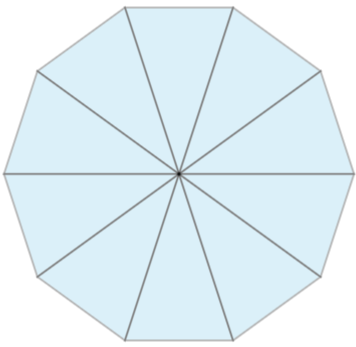
\includegraphics[bb=0 0 356 347,clip,width=3cm]{figures/initPenrose.png}
  \hspace{2cm}
  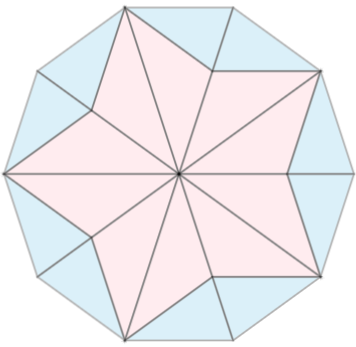
\includegraphics[bb=0 0 356 347,clip,width=3cm]{figures/div1.png}

  \vspace{1cm}
  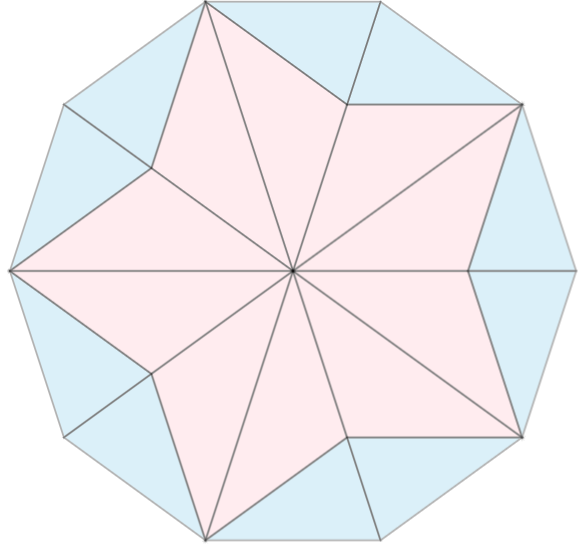
\includegraphics[bb=0 0 580 546,clip,width=5cm]{figures/div1inf1.png}
  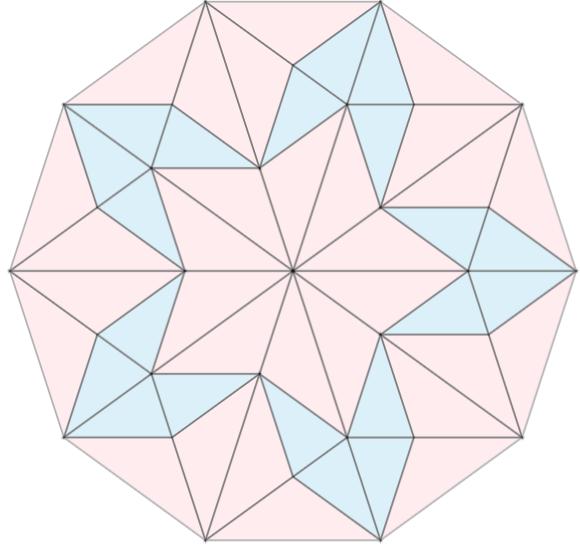
\includegraphics[bb=0 0 580 546,clip,width=5cm]{figures/div2.png}

  \vspace{1cm}
  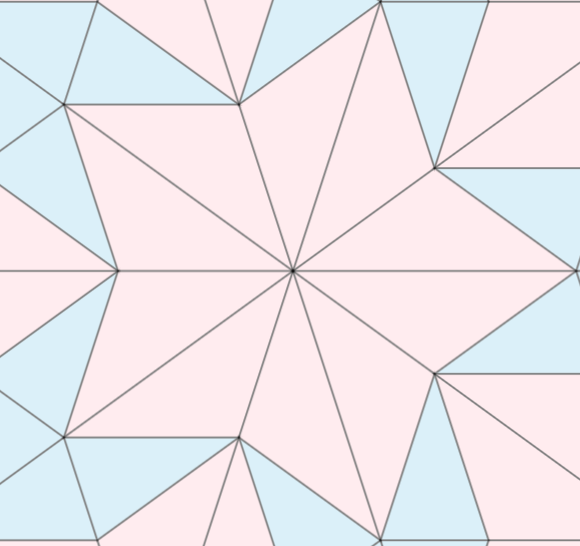
\includegraphics[bb=0 0 580 546,clip,width=5cm]{figures/div2inf2.png}
  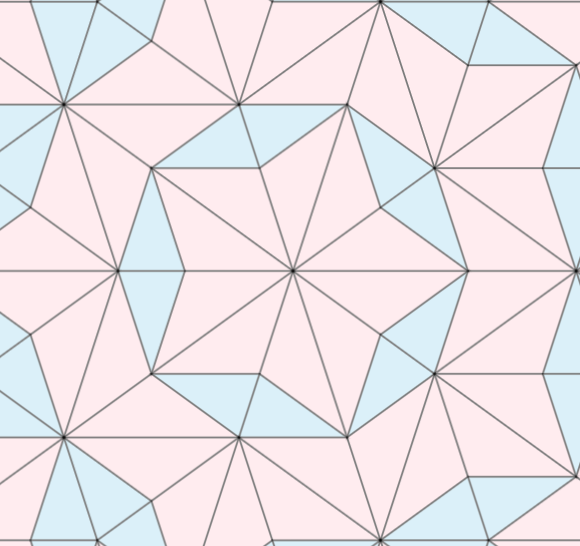
\includegraphics[bb=0 0 580 546,clip,width=5cm]{figures/div3.png}

  \vspace{1cm}
  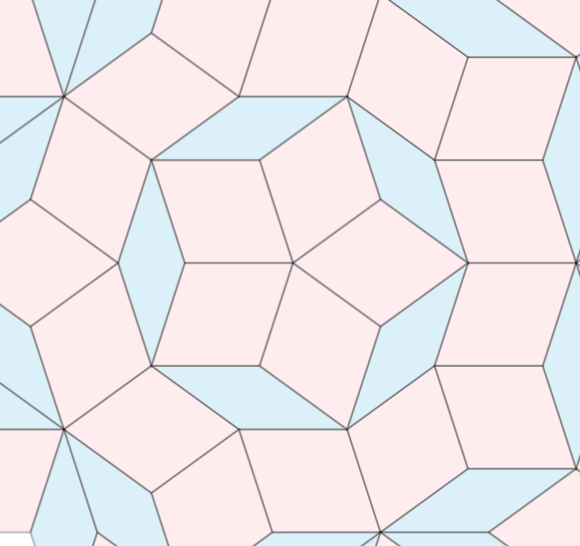
\includegraphics[bb=0 0 580 546,clip,width=5cm]{figures/unified.png}

  \caption{ペンローズタイル張りの構成の様子}
  \label{fig:penroseConstruction}
 \end{center}
\end{figure}


%以上の動きをペンローズタイル上でも行う。ペンローズタイルとは〜
ペンローズ・タイル張りにおいて各タイルを頂点とみなし、
辺で接するタイル同士が一本の辺で結ばれているグラフと考えると
各頂点の次数が$4$の正則グラフが得られる。
このグラフの上で砂山模型の実験を行った。

まずペンローズタイル上で雪崩を1000回発生させると以下のようになった。
\begin{center}
\includegraphics[width=10cm]{sand1000.pdf}
\end{center}
正方格子上での広がり方は〜角形に広がるが(図がほしい)、ペンローズタイル上での広がり方は円状に広がる。

規模と頻度の対数をそれぞれとってグラフにすると以下のようになる。

\begin{thebibliography}{99}
 \bibitem{BTW} P.Bak, C. Tang, and K. Wiesenfeld. {\em Self-organized criticality: An explanation of the 1/f noise.} 
	 Physical review letters 59.4 381, 1987.
\end{thebibliography}


\end{document}
